\section{Methodology}\label{sec:method}

Analizowaliśmy nie tylko kod, ale również powiązane z nim metadane. Proces badawczy składał się z czterech etapów: wyboru wersji AIDev, wzbogacenia profili deweloperów o dane aktywności z GitHub, podziału użytkowników na grupy oraz porównania korzystania z agentów pomiędzy tymi grupami. Wyniki na poziomie pull requestów zostały zagregowane per programista, by uniknąć traktowania wielu wkładów tej samej osoby jako niezależnych obserwacji.

\subsection{Data sources and sample construction}

Korzystamy z wydania Zenodo v3 zbioru AIDev (DOI \texttt{10.5281/zenodo.16919272}), opisanego w Sekcji 1.

Aktywność w AIDev opisuje deweloperów głównie w odniesieniu do wkładu powiązanego z agentami. Aby uzyskać szerszy zakres informacji, wzbogaciliśmy rekordy za pomocą GitHub GraphQL API. Tabela~\ref{tab:profile-indicators} przedstawia 12 ilościowych wskaźników użytych do klastrowania. Wskaźniki pięcioletnie obejmują pięć lat poprzedzających zbieranie danych. GitHub udostępnia tylko zagregowaną liczbę kontrybucji do prywatnych repozytoriów (nie tylko commitów, i tylko dla użytkowników, którzy zgodzili się to pokazywać) - nie należy tego interpretować jako dokładną liczbę prywatnych commitów. W procesie gromadzenia danych login uznawano za niedostępny - usunięty, przemianowany lub z jakiegoś innego powodu niedostępny - gdy API zwróciło status inny niż 200. Odpowiadający im deweloperzy to dokładnie ci, których wskaźniki później oszacowano metodą lasu losowego, opisaną poniżej. Zbieranie danych GraphQL przeprowadzono 6 maja 2026 roku. Należy zwrócić uwagę, że jest to około 9 miesięcy po okresie, którego dotyczą dane z AIDev, i mogły one ulec zmianie w tym czasie.

Zbieranie danych GraphQL dało rekordy aktywności dla 70\,434 z 72\,189 deweloperów (97,57\%). Wskaźniki liczbowe pozostałych 1755 deweloperów oszacowano za pomocą modeli regresji lasu losowego \cite{breiman2001random}. Modele oceniono przy podziale 80/20 na zbiór treningowy i testowy, a przewidziane wartości liczbowe zaokrąglano do liczb całkowitych. Ich skuteczność predykcyjna była ograniczona - obserwowane wartości $R^2$ przedstawia Tabela~\ref{tab:r2-values}. Wartości te należy więc traktować jako przybliżone uzupełnienie brakujących profili, a nie wiarygodną rekonstrukcję ich aktywności.

\begin{table}[tb]
    \centering
    \caption{Skuteczność predykcyjna ($R^2$) modeli imputacji lasem losowym.}
    \label{tab:r2-values}
    \small
    \begin{tabular}{lr}
        \toprule
        \textbf{Wskaźnik} & \textbf{$R^2$} \\
        \midrule
        \texttt{collab\_breadth} & 0,098 \\
        \texttt{5yr\_prs\_opened} & 0,088 \\
        \texttt{5yr\_reviews\_given} & 0,020 \\
        \texttt{5yr\_public\_commits} & $-0{,}073$ \\
        \texttt{5yr\_private\_work} & $-0{,}272$ \\
        \bottomrule
    \end{tabular}
\end{table}
\begin{table}[tb]
    \centering
    \caption{Wskaźniki użyte do wyznaczenia profili aktywności deweloperów.}
    \label{tab:profile-indicators}
    \small
    \begin{tabularx}{\linewidth}{@{}p{0.31\linewidth}X@{}}
        \toprule
        \textbf{Wskaźnik} & \textbf{Operacjonalizacja} \\
        \midrule
        Zakres współpracy & Liczba repozytoriów, do których deweloper wniósł wkład. \\
        Publiczne commity & Publiczne kontrybucje typu commit w ciągu poprzedzających pięciu lat. \\
        Aktywność zastrzeżona & Zastrzeżone kontrybucje w ciągu poprzedzających pięciu lat, gdy ujawnione przez GitHub. \\
        Otwarte pull requesty & Pull requesty otwarte w ciągu poprzedzających pięciu lat. \\
        Złożone recenzje & Recenzje pull requestów złożone w ciągu poprzedzających pięciu lat. \\
        Staż konta & Czas, jaki upłynął od utworzenia konta GitHub. \\
        Obserwujący & Liczba obserwujących w momencie zbierania danych. \\
        Maksymalna liczba gwiazdek & Największa liczba gwiazdek wśród repozytoriów należących do dewelopera. \\
        Maksymalna liczba forków & Największa liczba forków wśród repozytoriów należących do dewelopera. \\
        Rozpiętość aktywności Agentic-PR & Liczba dni między pierwszym a ostatnim Agentic-PR dewelopera. \\
        Różnorodność agentów & Liczba różnych agentów kodujących użytych w Agentic-PR dewelopera. \\
        Zakres repozytoriów Agentic-PR & Liczba różnych repozytoriów, w których deweloper ma Agentic-PR. \\
        \bottomrule
    \end{tabularx}
\end{table}

\subsection{Preprocessing and activity-profile construction}

Wskaźniki były silnie prawoskośne i różniły się o kilka rzędów wielkości. Zastosowaliśmy transformację log(1+x), a następnie wystandaryzowaliśmy każdą cechę do średniej zero i wariancji jeden. Następnie użyliśmy Isolation Forest z parametrem kontaminacji ustawionym na 1\%, aby usunąć najbardziej skrajne przypadki \cite{liu2008isolation}. W wyniku tej procedury usunięto 722 programistów, pozostawiając 71\,467 profili do głównej analizy.

Transformację kwantylową w kierunku rozkładu normalnego brzegowego wypróbowano najpierw zamiast log(1+x), ale kontrola wrażliwości typu complete-case (Sekcja 5) wykazała jej niestabilność. Klastrowanie na danych zawierających wyłącznie deweloperów z rzeczywistymi danymi GraphQL zgadzało się z klastrowaniem pełnej populacji jedynie przy Adjusted Rand Index = 0,46. Ta sama kontrola z log(1+x) dała Adjusted Rand Index = 0,98, więc pozostano przy tej drugiej metodzie.

Analizę głównych składowych obliczono na przekształconych wskaźnikach, aby wspomóc interpretację dominujących osi zmienności, a nie jako etap redukcji wymiarowości zasilający algorytm klastrowania \cite{jolliffe2016principal}. Pierwsze dwie główne składowe zachowują jedynie około 50\% wariancji, więc projekcja do 2 wymiarów odrzucałaby mniej więcej połowę informacji. Dlatego klastrowanie przeprowadziliśmy na pełnej, 12-wymiarowej, oczyszczonej reprezentacji; PCA(2) raportujemy osobno, wyłącznie w celu wizualizacji, które wskaźniki napędzają dwie dominujące osie. Jak pokazuje Rysunek~\ref{fig:pca-loadings}, pierwsza składowa ładuje się dodatnio na wskaźnikach aktywności i można ją interpretować jako oś ogólnej aktywności. Druga składowa przeciwstawia aktywność powiązaną z agentami i wielkość wkładu publicznego ogólnej rozpoznawalności oraz aktywności recenzenckiej.

\begin{figure}[tb]
    \centering
    
\includegraphics[width=0.92\linewidth]{pca_1.png}
    \vspace{0.5em}
    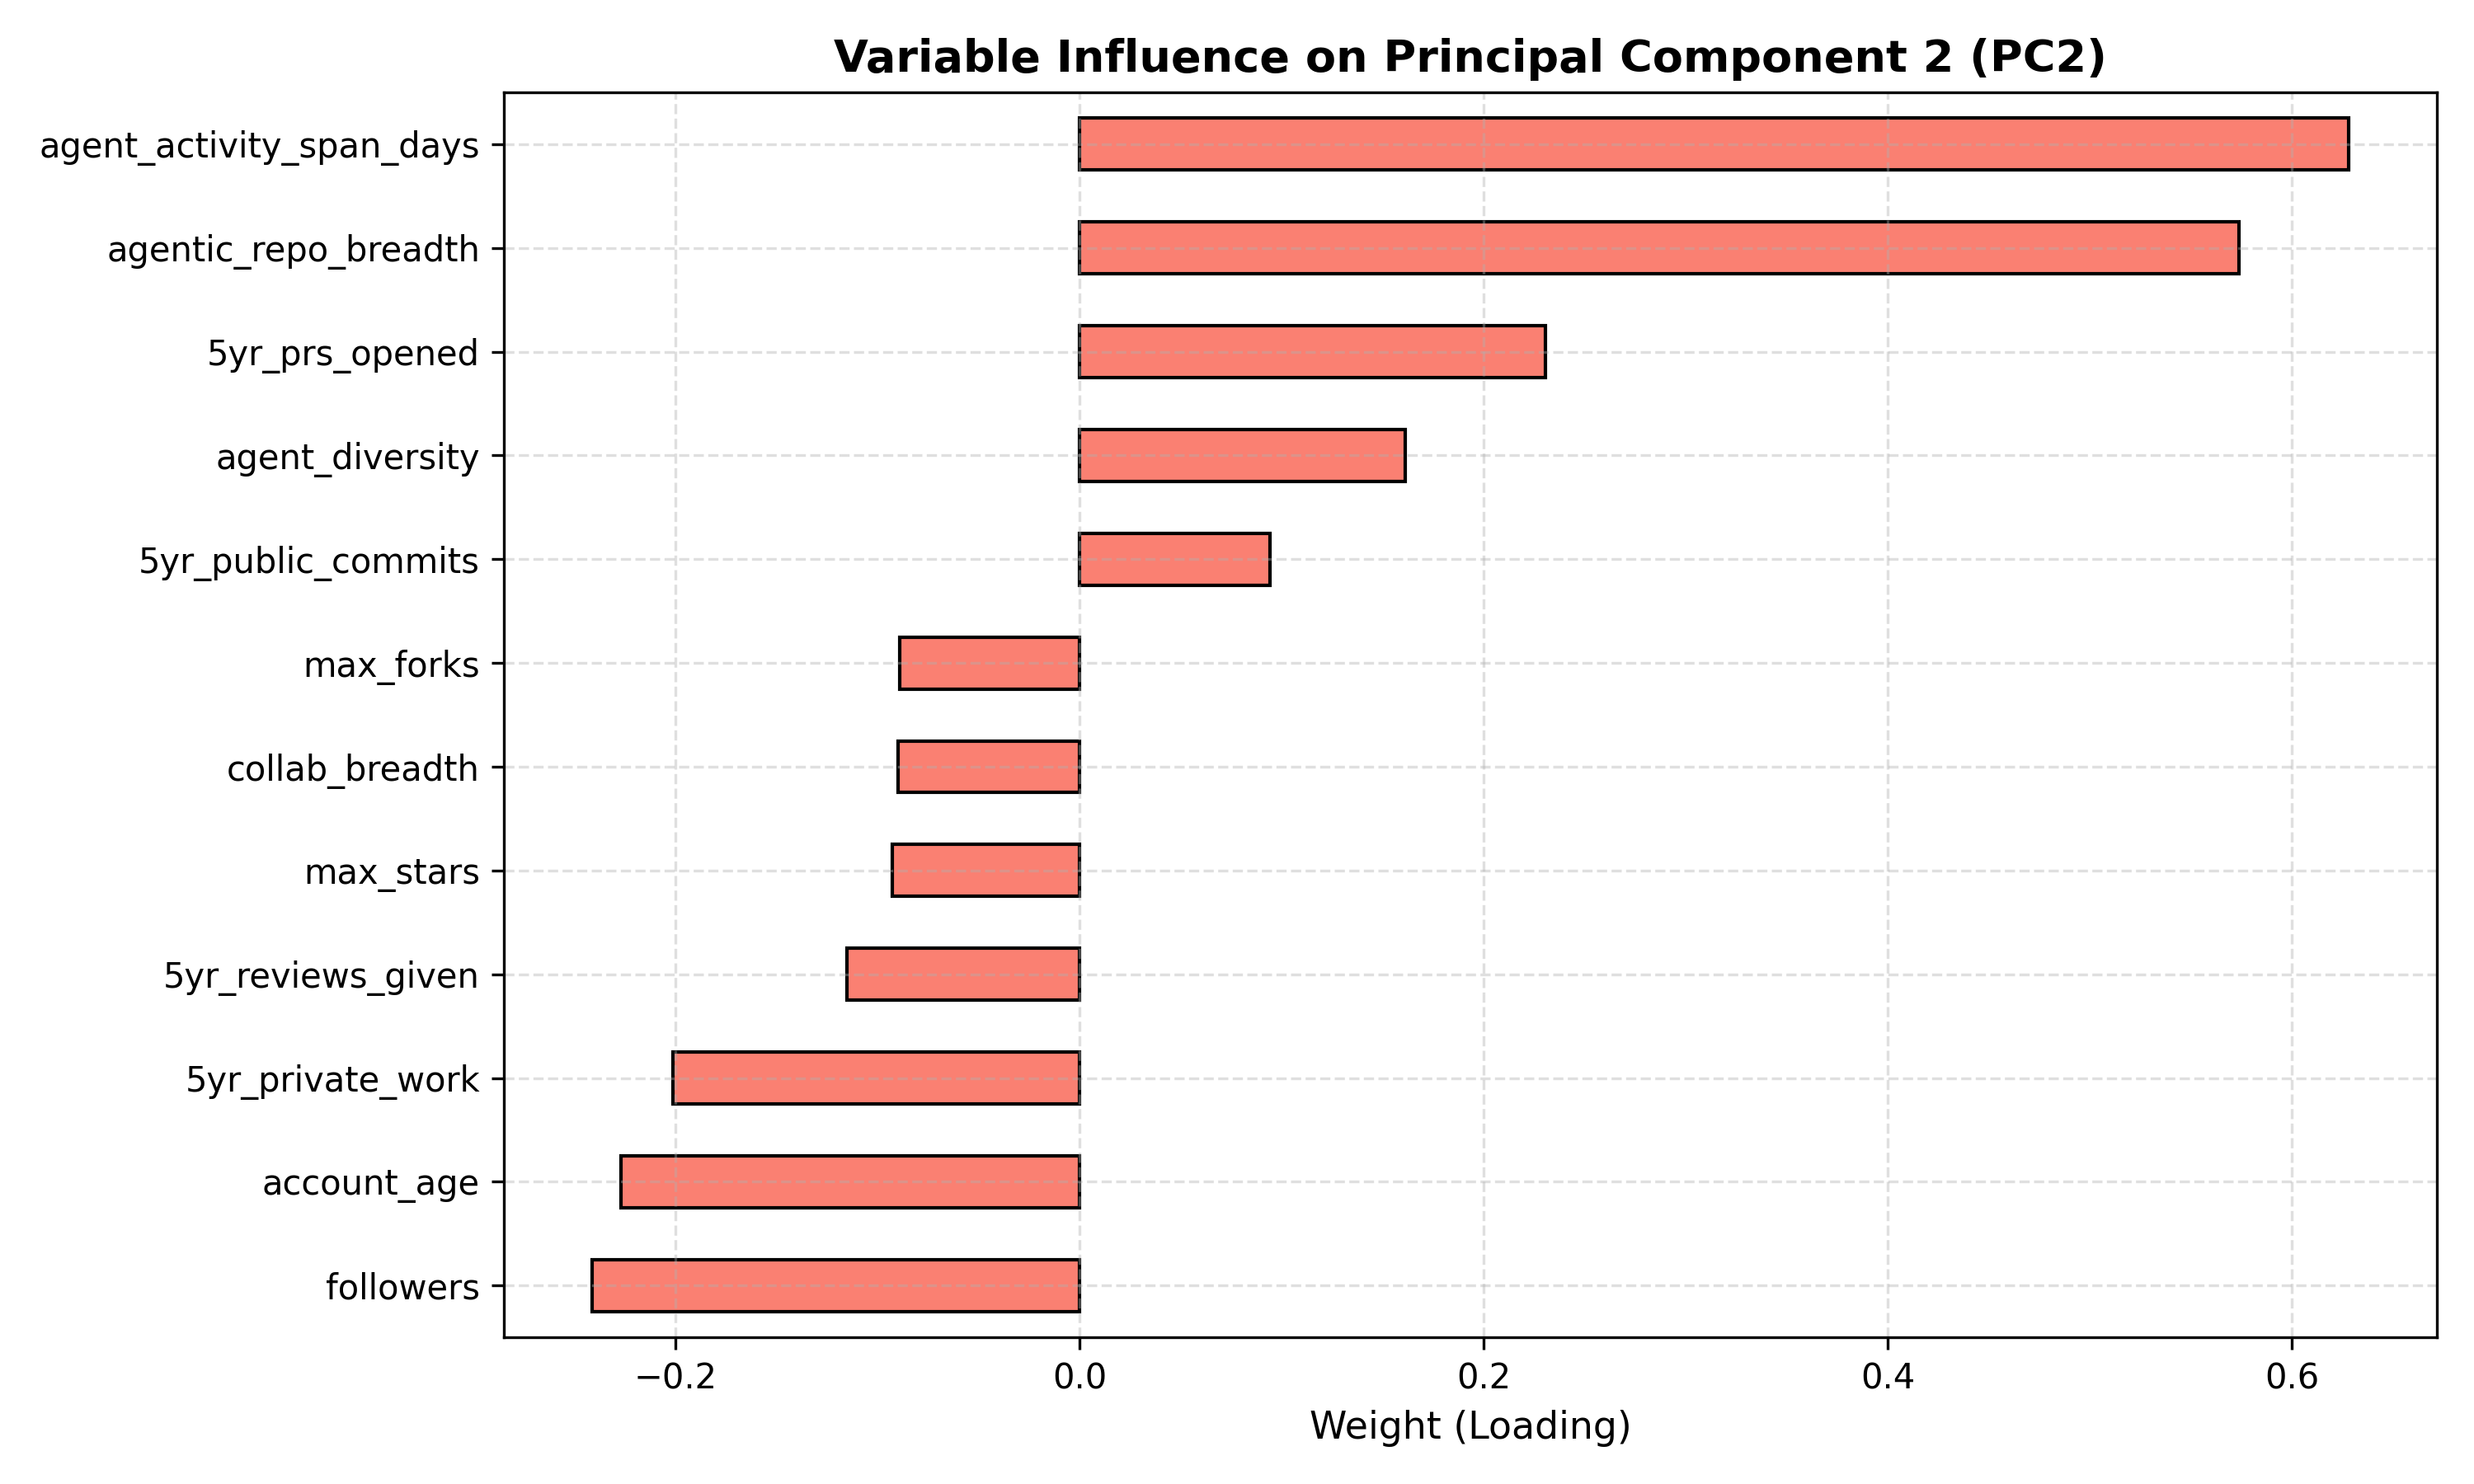
\includegraphics[width=0.92\linewidth]{pca_2.png}
    \caption{Ładunki wskaźników aktywności na dwóch dominujących osiach zmienności (PC1, PC2), obliczone wyłącznie w celach interpretacyjnych; PC1+PC2 zachowują około 50\% wariancji i nie są używane jako dane wejściowe do klastrowania. PC1 reprezentuje przede wszystkim ogólną aktywność na GitHub, podczas gdy PC2 przeciwstawia aktywność powiązaną z agentem i wielkość wkładu publicznego ogólnej rozpoznawalności i aktywności recenzenckiej.}
    \label{fig:pca-loadings}
\end{figure}

Pełną, 12-wymiarową, oczyszczoną reprezentację podzieliliśmy za pomocą klastrowania $k$-średnich \cite{lloyd1982least}. Zbadaliśmy również rezultaty dla różnych wartości $k=2,\ldots,10$ przy użyciu average silhouette width \cite{rousseeuw1987silhouettes} oraz gap statistic \cite{tibshirani2001gap}, obliczonych na tej samej 12-wymiarowej reprezentacji. Rysunek~\ref{fig:cluster-diagnostics} pokazuje, że $k=3$ nie jest optimum liczbowym według żadnej z tych statystyk. Mimo to zachowaliśmy $k=3$ jako celowo uproszczony i interpretowalny parametr, dopasowany do porównań pomiędzy profilami o niskiej, pośredniej i wysokiej aktywności. Analiza jest więc warunkowa względem tego wyboru i nie zakłada, że trzy klastry stanowią wewnętrzną strukturę populacji deweloperów.

\begin{figure}[tb]
    \centering
    
\includegraphics[width=0.90\linewidth]{silnouette.png}
    \vspace{0.5em}
    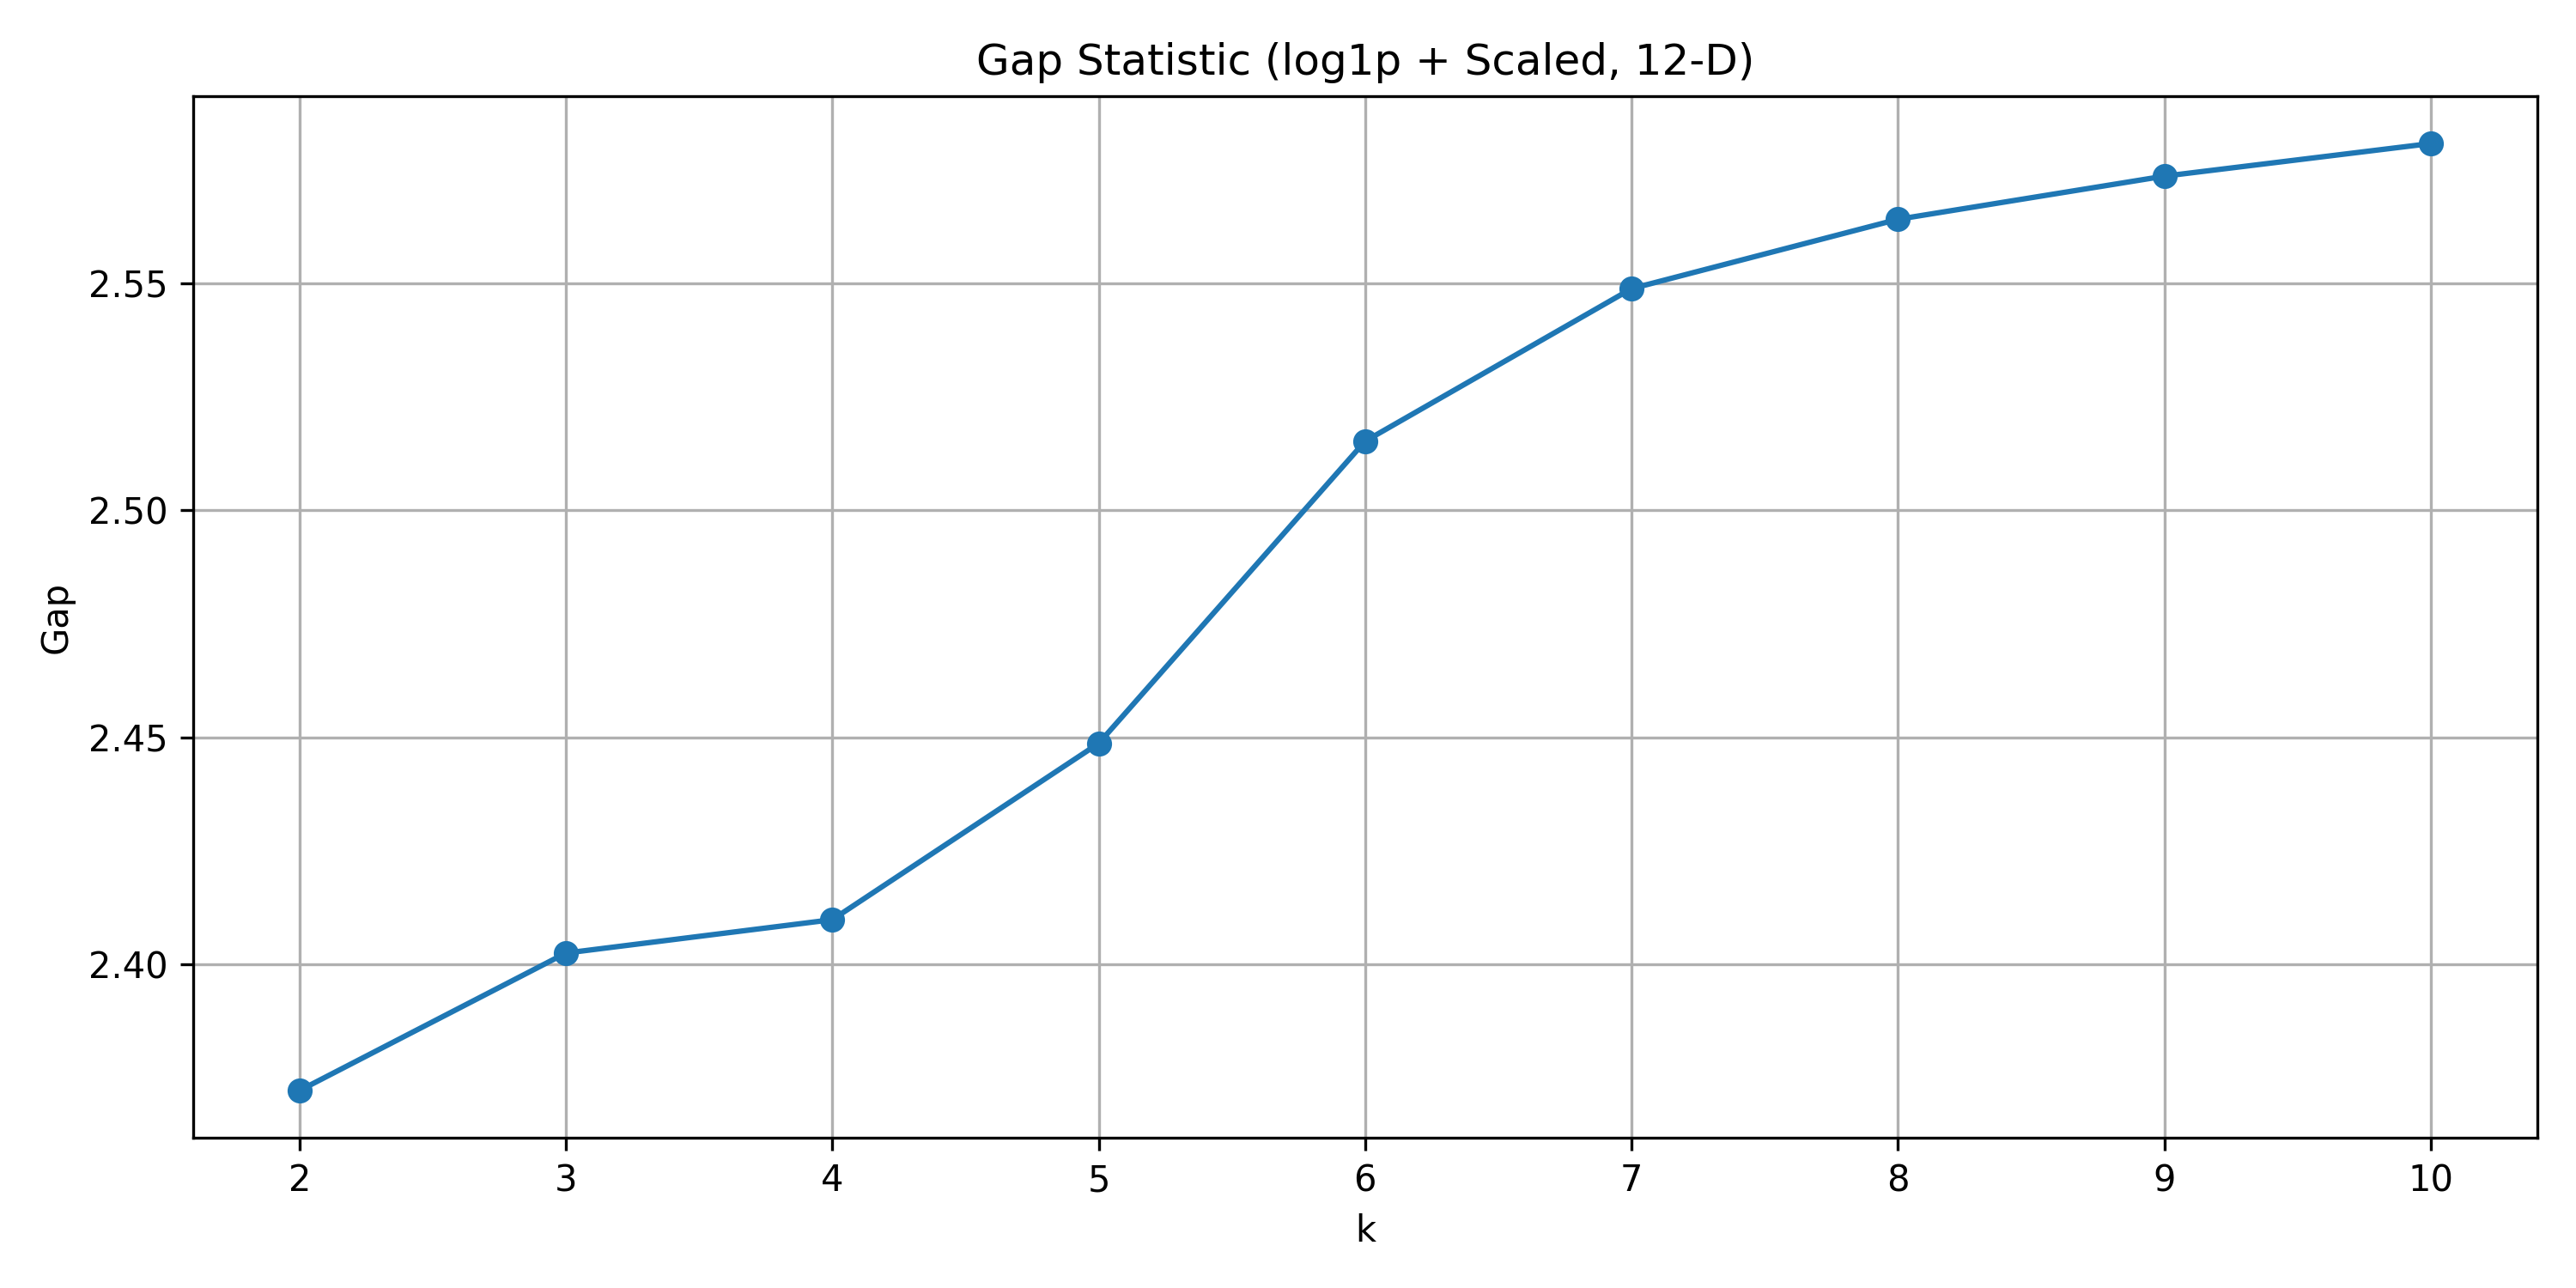
\includegraphics[width=0.90\linewidth]{gap_statistic.png}
    \caption{Diagnostyki szerokości sylwetki i statystyki luki dla kandydujących wartości $k$, obliczone na 12-wymiarowych danych wejściowych klastrowania. $k=3$ nie jest optimum liczbowym według żadnej z diagnostyk; jest zachowane jako wybór projektowy podyktowany interpretowalnością.}
    \label{fig:cluster-diagnostics}
\end{figure}

Dla czytelności profile o niskiej, pośredniej i wysokiej aktywności nazywamy odpowiednio \emph{Junior}, \emph{Mid} i \emph{Senior}. Liczą one odpowiednio 44\,854, 12\,705 i 13\,908 deweloperów. Te etykiety nie są zweryfikowanymi stanowiskami zawodowymi, etapami kariery ani bezpośrednimi pomiarami kompetencji programistycznych. Ta rozbieżność ma konkretne znaczenie dla RQ1: profil Mid okazuje się mieć najwyższą medianę liczby Agentic-PR spośród trzech profili (Sekcja~\ref{sec:results}), mimo że w rankingu złożonego wyniku aktywności plasuje się niżej niż Senior, ponieważ ten wynik odzwierciedla też wskaźniki (obserwujący, staż konta, gwiazdki i forki repozytoriów), na których Senior wypada wyżej.

\subsection{Outcome measures}

Zmienne wynikowe nie były uwzględnione wśród danych wejściowych klastrowania.

\paragraph{RQ1: AI-agent use intensity.}
Dla każdego dewelopera policzyliśmy liczbę Agentic-PR powiązanych z tym deweloperem w pełnym zbiorze danych AIDev. Zmienna ta mierzy obserwowaną wielkość wkładu w oknie czasowym zbioru danych. Nie mierzy natomiast udziału całkowitej pracy dewelopera wykonanej z użyciem agenta ani ogólnego prawdopodobieństwa, że deweloper korzysta z narzędzi AI.

\paragraph{RQ2: pull-request acceptance.}
Dla każdego dewelopera obliczyliśmy proporcję rozstrzygniętych Agentic-PR, które zostały scalone. Pull request klasyfikowano jako scalony, gdy jego pole \texttt{merged\_at} było niepuste, a jako odrzucony, gdy został zamknięty bez scalenia. Otwarte pull requesty wykluczono z mianownika, zamiast traktować je jako odrzucone. Deweloperów bez rozstrzygniętego Agentic-PR wykluczono z tej analizy. Ten wynik dotyczy akceptacji pull requestów, a nie poprawności poszczególnych wygenerowanych linii kodu ani ogólnej jego jakości.

\paragraph{RQ3: Agentic-PR acceptance vs.\ a human-authored baseline.}
AIDev osobno udostępnia tabelę \texttt{human\_pull\_request} - bazową próbę pull requestów autorstwa ludzi (bez udziału agenta), pochodzącą z repozytoriów z ponad 500 gwiazdkami. Rozważaliśmy początkowo programistów znajdujących się w obu tych grupach, ale okazało się, że jedynie 351 z 2515 odrębnych autorów w \texttt{human\_pull\_request} znalazło się jednocześnie wśród 72\,189 deweloperów powiązanych z Agentic-PR. Stąd decyzja, że w RQ3 porównujemy dwie niezależne populacje: wskaźnik akceptacji wszystkich Agentic-PR, zsumowany po profilach aktywności, w porównaniu do wskaźnika akceptacji \texttt{human\_pull\_request}, przy użyciu tej samej klasyfikacji scalony/odrzucony/otwarty co w RQ2. Jest to porównanie na poziomie populacji, a nie dopasowane na poziomie deweloperów, a bazowa populacja jest sama w sobie ograniczona do węższej próby repozytoriów niż pełna populacja Agentic-PR.

\subsection{Statistical analysis}
Rozkłady zmiennych wynikowych nie dało się prosto porównać z popularnymi i znanymi rozkładami, a miary oparte na liczności zawierały wiele remisów oraz zer. Dla RQ1-RQ2, z których każde porównuje trzy profile aktywności, najpierw stosujemy test Kruskala-Wallisa, aby ocenić, czy rozkłady wyniku różnią się pomiędzy trzema grupami. Istotny wynik testu ogólnego jest uzupełniany dwustronnymi parami testów Manna-Whitneya $U$, przy czym trzy porównania parami dla każdego pytania badawczego korygujemy poprawką Bonferroniego, przy poziomie istotności $\alpha=0,05$. RQ3 porównuje tylko dwie niezależne grupy, więc stosujemy pojedynczy test Manna-Whitneya $U$, bez etapu testu ogólnego Kruskala-Wallisa i bez poprawki Bonferroniego.

Dla każdej grupy zanotowaliśmy liczność próby, średnią, odchylenie standardowe i medianę. Dodatkowo uzupełniamy wartości $p$ wielkościami efektu: epsilon-kwadrat dla testu Kruskala-Wallisa oraz korelacją rangowo-biseryjną dla porównań parami. Każdą wielkość efektu raportujemy wraz z 95\% przedziałem ufności uzyskanym metodą nieparametrycznego bootstrapu: dla epsilon-kwadrat losujemy ponownie każdą grupę niezależnie ze zwracaniem, przeliczamy statystykę Kruskala-Wallisa i bierzemy 2,5. oraz 97,5. percentyl z 2000 powtórzeń losowania. Ta sama procedura, zastosowana do dwóch porównywanych grup, jest używana dla każdej korelacji rangowo-biseryjnej w porównaniach parami. Wszystkie analizy dotyczą związków pomiędzy profilami opartymi na aktywności a obserwowanymi wynikami.
